\documentclass[runningheads]{llncs}
\usepackage[T1]{fontenc}
\usepackage{newtxtext}
\usepackage[varvw]{newtxmath}
\usepackage{graphicx,booktabs,tikz,xcolor,multirow}
\usepackage[hidelinks]{hyperref}
\hypersetup{pdfauthor={Dang Truong Minh Le},pdftitle={When Fundus Classifiers Meet a New Source: The FundusShift Benchmark and a Low-Capacity Baseline}}
\usetikzlibrary{positioning,fit,arrows.meta,calc}
\renewcommand\UrlFont{\color{blue}\rmfamily}
\urlstyle{rm}
\emergencystretch=2em
\renewcommand{\topfraction}{.92}\renewcommand{\bottomfraction}{.6}\renewcommand{\textfraction}{.06}\renewcommand{\floatpagefraction}{.85}
\setcounter{topnumber}{3}\setcounter{totalnumber}{5}
\newcommand{\sups}[1]{Suppl.~S#1}
\begin{document}

\title{When Fundus Classifiers Meet a New Source: The FundusShift Benchmark and a Low-Capacity Baseline}
\titlerunning{The FundusShift Benchmark}
\author{Dang Truong Minh Le}
\authorrunning{D. T. M. Le}
\institute{Mohamed bin Zayed University of Artificial Intelligence, Abu Dhabi, United Arab Emirates\\ \email{dang.le@mbzuai.ac.ae}}
\maketitle

\begin{abstract}
A fundus classifier that excels on validation may fail on images from a new source, and so may its confidence scores. FundusShift is a leakage-controlled benchmark of normal, diabetic retinopathy (DR) and glaucoma images from fifteen public collections, with seven held-out test sources and a separate glaucoma-screening set. Under one protocol we evaluate 818 configurations of fine-tuned, frozen, prompt-based and domain generalization models, plus four multimodal LLMs, and repeat the key analyses over 50 random source rotations. Validation scores barely rank fine-tuned models at unseen sources (Spearman 0.05). Thresholds and conformal quantiles tuned on development data break their promises at new sources. Glaucoma, present in only two development sources, is the weakest class. We then propose LOTUS, leave-one-source-out linear heads on frozen MedSigLIP mean patch tokens fused with zero-shot text scores. Over the 50 rotations, with three seeds each, LOTUS reached a balanced accuracy of 0.789 against 0.746 for the strongest probe (higher on 43 of 50) and an expected calibration error of 0.034 against 0.084 (lower on 47 of 50). Its design used held-out results, so these are not untouched estimates. A probe fused with the same text scores came within 0.012 and the bag was no better than seed ensembling: the gain lies in the head recipe and text fusion, and removing between-site directions, part of our initial design, lowers accuracy. Fitting thresholds on leave-one-source-out predictions kept a 10\% risk target on 42 of 50 rotations instead of 19. On Messidor-2, an external DR cohort, LOTUS kept its DR ranking (AUROC 0.823) and was better calibrated than the probe and fine-tuned models. Fundus benchmarks should report results per source and class, and check reliability promises at unseen sources.
\noindent\textbf{Code, results and supplement:} \url{https://github.com/dangaura-tech/fundusshift} (archived at \url{https://doi.org/10.5281/zenodo.23911966}); \textbf{data and splits:} \url{https://huggingface.co/datasets/le-dang1haha/FundusShift}

\keywords{Fundus photography \and Source shift \and Benchmark \and Calibration \and Foundation models \and Glaucoma.}
\end{abstract}

\section{Introduction}
Diabetic retinopathy (DR) and glaucoma affect large populations worldwide, and fundus photography offers a low-cost way to screen for them. Deep models reach high accuracy within a study population, yet performance can drop at new sites. A screening tool must also \emph{know} when it may be wrong, but its thresholds and confidence scores are tuned during development and degrade under shift.

Evidence for fundus images leaves three gaps. Domain generalization (DG) studies usually target one disease and measure accuracy alone~\cite{drgen,gdrnet}. General DG benchmarks found that specialized algorithms rarely beat well-tuned empirical risk minimization~\cite{domainbed,wilds}. Foundation models~\cite{retfound,flair,medgemma} are often evaluated where pretraining may overlap with test data; we found such overlap for FLAIR on five of our eight held-out sources. No shared protocol answers a practical question: \emph{which approach, if any, keeps both its accuracy and its reliability at a source it has never seen?}

Our contributions are:
\begin{itemize}
\item \textbf{FundusShift}, a three-class benchmark from fifteen public collections, with leakage groups, source-held-out test data, a separate glaucoma-screening set and dedicated calibration splits (Sec.~\ref{sec:bench}).
\item \textbf{A reliability-first evaluation} of 818 configurations (25 encoders, ten method families; Table~\ref{tab:cover}) and four multimodal LLMs, covering raw and calibrated scores, selective prediction, conformal sets and 50 source rotations (Sec.~\ref{sec:diag}). Validation rank, calibration and risk control do not reliably transfer, and glaucoma drives much of the failure.
\item \textbf{LOTUS}, a low-capacity method on a frozen encoder that is more accurate and better calibrated than the linear and 16-shot probes over the rotations and more accurate than every representative on the published split (design informed by held-out results, as disclosed) (Secs.~\ref{sec:lotus} and~\ref{sec:eval}). A full factorial ablation shows that its head recipe and text fusion carry the gain, while the bag and the token input add little, and why explicit removal of site directions does not transfer.
\item \textbf{A shift-aware reference for promises}: thresholds fitted on leave-one-source-out predictions instead of in-distribution calibration data keep a risk target far more often, at a known cost in coverage (Sec.~\ref{sec:cert}).
\end{itemize}

\begin{figure}[tb]
\centering
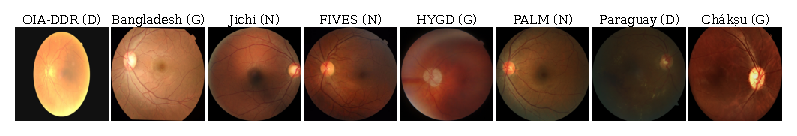
\includegraphics[width=\textwidth]{figures/samples.pdf}
\caption{Images from eight public sources (class in brackets), showing differences in field of view, colour and quality.}\label{fig:story}
\end{figure}

\section{Related Work}
\textbf{Domain generalization.} DRGen~\cite{drgen} and GDRNet~\cite{gdrnet} address DR grading at unseen domains; we cover DR and glaucoma and measure reliability as well as accuracy. DomainBed and WILDS showed that model selection and realistic splits are decisive~\cite{domainbed,wilds}; we follow them and include Group DRO~\cite{groupdro}, CORAL~\cite{coral} and SWAD~\cite{swad}.

\textbf{Foundation and vision-language models.} RETFound~\cite{retfound}, FLAIR~\cite{flair}, BiomedCLIP~\cite{biomedclip} and MedSigLIP~\cite{medgemma} supply pretrained encoders, alongside general ones such as DINOv2~\cite{dinov2} and SigLIP~\cite{siglip}. We also test prompt learning~\cite{coop}, adapters~\cite{tip}, weight interpolation~\cite{wiseft} and multimodal LLMs~\cite{fundusr1}. Linear probing can outperform fine-tuning out of distribution~\cite{lpft}; we extend this observation to reliability. Heavier heads such as RPAttn~\cite{rpattn} improve multi-disease fundus classification within a dataset; we test whether they transfer.

\textbf{Reliability under shift.} Temperature scaling (TS)~\cite{guo2017}, focal temperature scaling (FTS)~\cite{fts} and calibration-aware losses~\cite{mdca,mbls} target better probabilities. Selective classification~\cite{sgr} and conformal prediction~\cite{lac} control risk and coverage under exchangeability, which a new site breaks; calibrating on held-out training domains improves calibration under shift~\cite{wald2021}, which our leave-one-source-out reference applies to thresholds. Test-time adaptation~\cite{tent,t3a} and prior-shift estimation~\cite{saerens} correct for shift without labels.

\textbf{Nuisance removal.} Nuisance attribute projection removes channel directions in speaker recognition~\cite{nap}. Our initial design adapted it to acquisition sites; we show that it erases task-correlated directions here and drop it. Each component of LOTUS is known; we did not find their combination in fundus work (our search was not systematic).

\section{The FundusShift Benchmark}\label{sec:bench}
\begin{table}[tb]
\caption{FundusShift sources and images by class: normal (N), diabetic retinopathy (D), glaucoma (G). Development (Dev) sources are split into train, validation and calibration. A further 861 out-of-scope images form an open-set probe (\sups{7}).}\label{tab:data}
\centering\scriptsize\setlength{\tabcolsep}{4pt}
\begin{tabular}{@{}lllrrrr@{}}
\toprule
Role & Source & Region & N & D & G & Total\\
\midrule
Dev & Bangladesh Eye~\cite{bangladesh} & South Asia & 846 & 1,500 & 1,156 & 3,502 \\
Dev & OIA-DDR~\cite{ddr} & East Asia & 6,265 & 6,255 & -- & 12,520 \\
Dev & DeepDRiD~\cite{deepdrid} & East Asia & 914 & 1,086 & -- & 2,000 \\
Dev & GRAPE~\cite{grape} & East Asia & -- & -- & 586 & 586 \\
Dev & IDRiD~\cite{idrid} & South Asia & 167 & 347 & -- & 514 \\
Dev & Jichi~\cite{jichi} & East Asia & 6,295 & 3,120 & -- & 9,415 \\
Dev & SUSTech-SYSU~\cite{sustech} & East Asia & 631 & 588 & -- & 1,219 \\
\midrule
Test & AFIO~\cite{afio} & South Asia & 67 & 18 & 44 & 129 \\
Test & FIVES~\cite{fives} & East Asia & 193 & 200 & 193 & 586 \\
Test & HRF~\cite{hrf} & Europe & 15 & 15 & 15 & 45 \\
Test & HYGD~\cite{hygd} & Middle East & -- & -- & 548 & 548 \\
Test & PALM~\cite{palm} & East Asia & 161 & -- & -- & 161 \\
Test & PAPILA~\cite{papila} & Europe & 333 & -- & 87 & 420 \\
Test & Paraguay~\cite{paraguay} & Latin America & 708 & 723 & -- & 1,431 \\
\midrule
OOD & Ch\'ak\d{s}u~\cite{chaksu} & South Asia & 1,156 & -- & 187 & 1,343 \\
\bottomrule

\end{tabular}
\end{table}

\textbf{Data.} Table~\ref{tab:data} lists the sources, all publicly released; this is a secondary analysis under each source's licence, with labels used as published. Development data comprise 23,805 training, 2,983 validation and 2,968 calibration images. The test split holds 3,320 images from seven unseen sources, and Ch\'ak\d{s}u (1,343 images) is kept apart as a glaucoma-screening view. A source is one public collection: all but OIA-DDR (147 hospitals) come from a single institution or study, so held-out units are collections, not hospitals, and no acquisition institution spans development and test (\sups{1}). Two structural facts shape the results. G appears in only two development sources, and GRAPE holds nothing else, so a model can learn their appearance instead of the disease. Five of seven development sources graded only DR, so their ``normal'' means ``no DR'' (\sups{1}). Two test sources hold a single class (HYGD, PALM), for which bAcc reduces to recall; Sec.~\ref{sec:pub} reports results without them.

\textbf{Leakage control.} Exact hashes, vessel-pattern normalized cross-correlation and patient identifiers are joined into leakage groups, which never span two splits. This found, among others, brightness-altered copies of GRAPE photographs inside FIVES, which were removed. An automated audit confirms that no leakage group, file, patient, near-duplicate pair or acquisition family spans the development and test sides (\sups{1}).

\textbf{Protocol.} Validation selects checkpoints and hyperparameters; calibration subset Cal-A fits temperatures; Cal-B fits thresholds and conformal quantiles; test and Ch\'ak\d{s}u are used only for reporting. Each setting's \emph{representative} is its configuration with the highest validation balanced accuracy (bAcc), so test scores play no part in choosing baselines. Raw, TS and FTS scores pass through identical code. FLAIR is reported apart, since its pretraining names FIVES, HRF, PAPILA, Paraguay and Ch\'ak\d{s}u.

\textbf{Methods.} Table~\ref{tab:cover} summarizes the benchmark. Trained settings use three seeds; fine-tuning losses are cross-entropy, label smoothing, focal, MDCA~\cite{mdca} and MbLS~\cite{mbls}. Recipes were audited against pitfalls such as input-size mismatches (\sups{2}).

\begin{table}[tb]
\caption{Coverage of the benchmark on test, FLAIR excluded (reported apart). Configs: distinct (setting, encoder, configuration). Runs: including seeds. Selection: what validation chooses.}\label{tab:cover}
\centering\scriptsize\setlength{\tabcolsep}{2.5pt}
\resizebox{\textwidth}{!}{%
\begin{tabular}{@{}llrrl@{}}
\toprule
Setting & Encoders and options & Configs & Runs & Selection\\
\midrule
Fine-tuning & 13 CNN/ViT/RETFound~\cite{retfound} $\times$ 5 losses~\cite{mdca,mbls} & 65 & 195 & best epoch \\
Fine-tuning, NLL rule & Sensitivity check & 2 & 6 & best epoch, NLL \\
Linear probe & 25 encoders, 3 weightings, 5 losses & 375 & 1125 & best epoch \\
MLP probe & Frozen encoders & 11 & 33 & best epoch \\
16-shot probe & Frozen encoders, 16 per class & 125 & 375 & best epoch \\
Zero-shot & Vision-language encoders, 3 prompt banks & 33 & 33 & prompt bank \\
CoOp~\cite{coop} and variants & Vision-language encoders & 190 & 570 & fixed recipe \\
Tip-Adapter~\cite{tip} & Vision-language encoders & 6 & 18 & $\alpha,\beta$, bank \\
ERM, Group DRO~\cite{groupdro}, CORAL~\cite{coral}, SWAD~\cite{swad} & ConvNeXt-T~\cite{convnext}, DINOv2 LoRA~\cite{dinov2} & 7 & 21 & best epoch; SWAD: own rule \\
WiSE-FT~\cite{wiseft} & Vision-language encoders & 4 & 12 & $\alpha$, checkpoint \\
Multiple choice & 4 multimodal LLMs, e.g.~\cite{fundusr1}, 6 option orders & 4 & 4 & none \\
\bottomrule

\end{tabular}}
\end{table}

\textbf{Metrics and statistics.} We report pooled bAcc, equal-source bAcc (Eq-src), macro AUROC and class recalls; ECE with 15 bins, NLL and Brier score; and coverage, risk and false reassurance (disease answered normal) at thresholds frozen before testing. Paired comparisons use 2,000 bootstrap draws over leakage groups with Holm correction. We also retrain on 50 random 7/7 partitions of the 14 non-OOD sources (80/10/10 group split of the development side); these share sources, so we report means and win counts, not $p$-values.

\section{Diagnosis: What Breaks at an Unseen Source}\label{sec:diag}
\begin{figure}[tb]
\centering
\begin{minipage}{.43\textwidth}\centering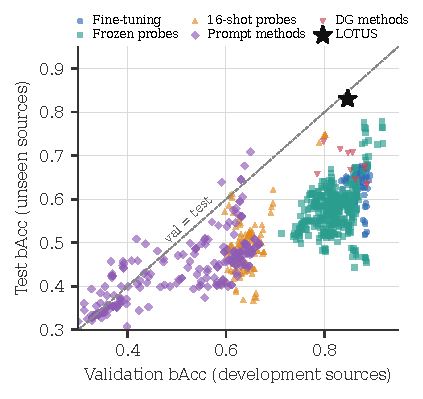
\includegraphics[width=\textwidth]{figures/val_test.pdf}\end{minipage}\hfill
\begin{minipage}{.56\textwidth}\centering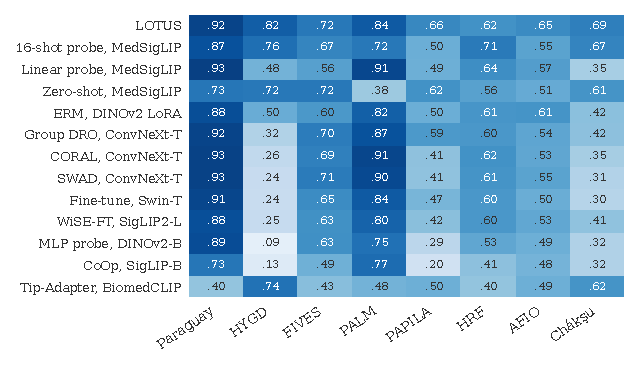
\includegraphics[width=\textwidth]{figures/heatmap.pdf}\end{minipage}
\caption{Left: validation against test bAcc for 816 configurations (FLAIR, multimodal LLMs and the two NLL-rule sensitivity runs excluded). Most points lie well below the diagonal, and the fine-tuning cluster is nearly flat. Right: bAcc per unseen source for LOTUS (Sec.~\ref{sec:lotus}) and the validation-selected representatives; single-class sources show recall.}\label{fig:val}
\end{figure}

\textbf{Finding 1: Validation is a weak guide to new sources.} Validation exceeded test bAcc in 94.5\% of configurations, with a median gap of 0.194 (Fig.~\ref{fig:val}, left). The Spearman correlation between validation and test bAcc was 0.786 overall, but this mostly reflects differences between families: within fine-tuning, whose validation scores span 0.85--0.89, it was 0.053, and on Ch\'ak\d{s}u it was negative ($-0.156$). The MedSigLIP linear probe had the highest validation bAcc among representatives (0.920) but reached 0.728 on test and 0.347 on Ch\'ak\d{s}u; fine-tuned Swin-T fell from 0.893 to 0.655 and 0.298.

\begin{figure}[tb]
\centering
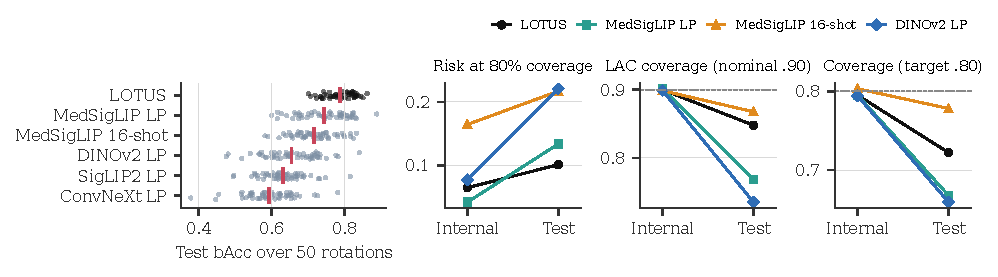
\includegraphics[width=\textwidth]{figures/rotation.pdf}
\caption{Fifty source rotations. Left: test bAcc per rotation, mean as a red bar; LP: linear probe. Right: internal estimates on held-back Cal-B against unseen test sources, means over rotations, after TS. Dashed lines mark the nominal target.}\label{fig:rot}
\end{figure}

\textbf{Finding 2: Reliability does not transfer.} Over 50 rotations and eight probe configurations (400 runs; Fig.~\ref{fig:rot}, right; \sups{6}), validation exceeded test in 98\% of runs, risk at the threshold for 80\% coverage exceeded its internal estimate in 89\%, and coverage of 90\% least-ambiguous (LAC) conformal sets~\cite{lac} fell below its internal estimate in 85\%. For the MedSigLIP linear probe, risk rose from 0.042 to 0.134 and LAC coverage fell from 0.901 to 0.769. Splitting Cal-B in half shows that the promises hold on unseen halves of the same sources, so the failure comes from the new sources, not from a small calibration set (\sups{5}). TS can harm an already calibrated model (linear probe: 0.024 to 0.079), FTS rarely improved on TS (\sups{3}), and a class-prior predictor has ECE 0.063, so ECE must be read with accuracy.

\textbf{Finding 3: Glaucoma is the weakest link.} Averaged over test sources, pairwise AUROC was 0.90--0.95 for N--D and D--G across the main representatives, but only 0.64--0.75 for N--G (\sups{6}). The difficulty is tied to shift rather than to the images alone: a logistic regression on frozen features reached a much higher bAcc when trained within each target source than when trained on development data (Table~\ref{tab:ceiling}), although AFIO stays low even within source. Site diversity is the bottleneck: over the rotations, recall G of the MedSigLIP linear probe rose from 0.468 with two glaucoma sources on the development side to 0.674 with four (LOTUS: 0.614 to 0.723). Models thus miss glaucoma or over-call it (\sups{4}).

\begin{table}[tb]
\caption{Trained on development sources against trained within the target source (cross-validated), logistic regression on frozen features, mean bAcc over nine encoders. Within-source learning can use source-specific cues, so it is a reference level, not a strict upper bound.}\label{tab:ceiling}
\centering\scriptsize
\begin{tabular}{@{}lrrrrrr@{}}
\toprule
& AFIO & Ch\'ak\d{s}u & FIVES & HRF & PAPILA & Paraguay\\
\midrule
Trained on development & .516 & .352 & .581 & .583 & .394 & .817\\
Trained within source & .635 & .718 & .857 & .779 & .757 & .928\\
\bottomrule
\end{tabular}
\end{table}

\textbf{Finding 4: There is no cheap fix.} DG losses did not close the gap: on ConvNeXt-T, Group DRO, CORAL and SWAD reached 0.707, 0.676 and 0.672 on test. Prompt-learning and adapter models (0.48--0.50) fell below plain zero-shot (0.709). Test-time adaptation (TENT~\cite{tent}, T3A~\cite{t3a}) gave no stable gain, and label-free prior estimation~\cite{saerens} was unstable: it lifted the linear probe to 0.835 but dropped zero-shot to 0.635; over rotations it cut LOTUS to 0.732 (\sups{9}), and label-free per-site feature standardization cut it to 0.685--0.692 (\sups{10}). Multimodal LLMs scored lowest (best: Fundus-R1~\cite{fundusr1}, 0.576).

A remedy must therefore generalize without target data and avoid fitting the appearance of the two glaucoma sources.

\section{LOTUS}\label{sec:lotus}
\begin{figure}[tb]
\centering
\resizebox{\textwidth}{!}{%
\begin{tikzpicture}[font=\footnotesize,>={Stealth[length=1.6mm]},
 b/.style={draw,rounded corners=1.5pt,minimum height=8mm,inner sep=3pt,align=center,fill=#1},b/.default=white]
\node[b=gray!12] (i) {Fundus\\image $x$};
\node[b=gray!12,right=5mm of i] (e) {MedSigLIP\\frozen};
\node[b,right=7mm of e,yshift=8mm] (t) {Mean patch\\token $\bar t(x)$};
\node[b=blue!10,right=4mm of t] (h) {Linear head $W_s$\\trained without\\source $s$};
\node[b=blue!10,right=4mm of h] (a) {Rescale;\\mean over\\$S$ heads};
\node[b,right=7mm of e,yshift=-9mm,minimum width=20mm] (v) {Image\\embedding};
\node[b=orange!15,right=4mm of v,minimum width=39mm] (p) {Similarity to three prompt\\banks; rescale; mean};
\node[circle,draw,inner sep=1pt,right=4mm of a,yshift=-8.5mm] (f) {$\tfrac12{+}\tfrac12$};
\node[b=gray!12,right=4mm of f] (o) {TS on\\Cal-A};
\node[b=gray!12,right=3mm of o] (y) {N, D, G};
\draw[->] (i)--(e); \draw[->] (e.east)--++(2mm,0)|-(t.west); \draw[->] (e.east)--++(2mm,0)|-(v.west);
\draw[->] (t)--(h); \draw[->] (h)--(a); \draw[->] (v)--(p);
\draw[->] (a.east)-|(f.north); \draw[->] (p.east)-|(f.south); \draw[->] (f)--(o); \draw[->] (o)--(y);
\end{tikzpicture}}
\caption{LOTUS (Leave-One-source-out Token heads Unified with zero-shot Scores). Only the linear heads are trained, about 8,000 parameters in all; the encoder (about 0.4B parameters) and prompt banks are fixed. Low capacity refers to the trained part only.}\label{fig:arch}
\end{figure}

LOTUS (Fig.~\ref{fig:arch}) follows one principle: \emph{where site support is thin, spend little capacity, and do not depend on any single source.} A linear head on frozen features cannot memorize much site appearance, bagging over left-out sources avoids depending on any one of them, and text scores do not depend on the training sites' class balance.

\textbf{Token input.} MedSigLIP~\cite{medgemma} takes a $448\times448$ image. We pool its last-layer patch tokens to a $14\times14$ grid, apply one fixed random orthonormal map to 384 dimensions (fitted on no data; it saved storage during development), and average over the grid to obtain $\bar t(x)$, standardized on training rows.

\textbf{Leave-one-source-out bag.} For each development source $s$ whose removal leaves all three classes ($S=7$ on the published split), we fit a linear head $W_s$ (1,155 parameters) on all other sources, with label smoothing 0.1, class-balanced sampling, AdamW (learning rate $3\times10^{-4}$, weight decay $10^{-2}$), batch size 64 and 12 epochs, keeping the epoch with the best validation bAcc on the head's own sites.

\textbf{Text fusion.} Three fixed prompt banks (a CLIP-style template ensemble, CuPL-style descriptions and one descriptive prompt; \sups{2}) give zero-shot logits $z_b^{\mathrm{text}}$ from MedSigLIP's image embedding. Let $\mathcal{R}$ centre a logit vector per image and divide it by its standard deviation over validation images. The final logits are
\begin{equation}
z(x)=\frac12\cdot\frac{1}{S}\sum_{s=1}^{S}\mathcal{R}\bigl(W_s\,\bar t(x)\bigr)+\frac12\cdot\frac13\sum_{b=1}^{3}\mathcal{R}\bigl(z^{\mathrm{text}}_b(x)\bigr).\label{eq:fusion}
\end{equation}
$\mathcal{R}$ puts both parts on one scale, so the equal weight needs no fitting, and prediction uses no target-source data. A temperature $T$ is fitted on Cal-A; averaging compresses logits, so $T<1$ is expected ($T=0.444$).

\textbf{Initial design: between-site projection.} Our initial design also removed, before each head, the directions along which development sites differ with class held fixed: with $\mu_{r,c}$ the mean of site $r$ and class $c$ on the head's training rows and $\mu_c$ the class mean, $U_s$ holds the leading right singular vectors of the stacked $\mu_{r,c}-\mu_c$ (at most 32; their rank gives 11--13 per head, 14 on all development data), and each head sees $(I-U_sU_s^{\top})\,\bar t(x)$.

\begin{table}[tb]
\caption{Development ablation of the initial design (leave-one-development-source-out, three seeds, equal-site mean; no test data). False G: non-glaucoma images predicted G (not recorded for text only).}\label{tab:abl}
\centering\scriptsize
\begin{tabular}{@{}lrrrrr@{}}
\toprule
Configuration & bAcc & ECE & NLL & Recall G & False G\\
\midrule
Single linear head on tokens & .689 & .128 & .717 & .608 & .164\\
Text only (three banks) & .758 & .245 & .749 & .605 & --\\
Bag + projection & .744 & .110 & .635 & .825 & .181\\
Single head + text & .759 & .133 & .616 & .650 & .098\\
Initial design: bag + projection + text & .792 & .151 & .575 & .764 & .100\\
\bottomrule
\end{tabular}
\end{table}

\textbf{Design and selection.} About 120 configurations were compared by leave-one-source-out on the seven development sources (\sups{8}). Heavier heads lost the G class at held-out sites (an RPAttn head~\cite{rpattn} on three token depths had recall G of 0.008), which led to the low-capacity design; on development data the projection raised recall G (Table~\ref{tab:abl}). Ten configurations reached a development bAcc of at least 0.791; all ten were evaluated on the published test split and the one with the highest test bAcc became the initial design (sixth on development; all ten reached 0.791--0.817, above the best test bAcc of any validation-selected representative, 0.748; \sups{9}). The rotation ablation of Sec.~\ref{sec:abl} then showed that the projection lowers accuracy, so LOTUS drops it and is otherwise unchanged. Both choices used held-out results. As a clean check, we re-selected the arm in every rotation by leave-one-source-out on its development side only: the selected models reached bAcc 0.780 against 0.746 for the probe (higher on 39 of 50) and ECE 0.035 against 0.084 (lower on 47 of 50; \sups{9}).

\section{Evaluating LOTUS}\label{sec:eval}
\subsection{Source Rotations}\label{sec:rot}
\begin{table}[tb]
\caption{Fifty source rotations, same partitions for all methods, TS on each rotation's Cal-A, one training seed per rotation. Risk: at the threshold for 80\% coverage fitted on Cal-B. LAC: coverage at nominal 0.90. LP: linear probe with class-weighted cross-entropy. Last four columns: LOTUS minus the row, and rotations where LOTUS is better. With three seeds, LOTUS against the MedSigLIP LP gives $+0.043$ bAcc (higher on 43/50) and lower ECE on 47/50 (\sups{6}).}\label{tab:rot}
\centering\scriptsize\setlength{\tabcolsep}{2.5pt}
\resizebox{\textwidth}{!}{%
\begin{tabular}{@{}lrrrrrrrrrrrr@{}}
\toprule
& & & \multicolumn{3}{c}{Recall} & & & & \multicolumn{4}{c}{LOTUS minus row}\\
\cmidrule(lr){4-6}\cmidrule(l){10-13}
Method & bAcc & Eq-src & N & D & G & ECE & Risk & LAC & $\Delta$bAcc & Higher & $\Delta$ECE & Lower\\
\midrule
\textbf{LOTUS} & .788 & .766 & .813 & .845 & .708 & .034 & .101 & .848 & -- & -- & -- & -- \\
MedSigLIP LP & .745 & .725 & .794 & .803 & .637 & .084 & .134 & .769 & +0.044 & 41/50 & -0.050 & 47/50 \\
MedSigLIP 16-shot & .716 & .713 & .685 & .742 & .723 & .056 & .217 & .868 & +0.072 & 49/50 & -0.022 & 36/50 \\
DINOv2 LP & .655 & .650 & .684 & .750 & .531 & .118 & .221 & .735 & +0.133 & 49/50 & -0.084 & 49/50 \\
SigLIP2 LP & .631 & .617 & .636 & .709 & .549 & .141 & .280 & .728 & +0.157 & 50/50 & -0.108 & 50/50 \\
ConvNeXt LP & .593 & .609 & .644 & .710 & .426 & .130 & .287 & .730 & +0.195 & 50/50 & -0.097 & 50/50 \\
\bottomrule

\end{tabular}}
\end{table}

LOTUS was retrained on each of the 50 partitions (Table~\ref{tab:rot}, Fig.~\ref{fig:rot} left). With three seeds, mean bAcc was 0.789 (5th--95th percentile 0.725--0.841); seeds changed it by 0.004, partitions by 0.039. Against the strongest baseline, the MedSigLIP linear probe, LOTUS gained $+0.043\pm0.049$ bAcc (higher on 43 of 50) with lower ECE after TS (0.034 against 0.084; lower on 47 of 50), and, with one seed (Table~\ref{tab:rot}), lower risk at the 80\%-coverage threshold (0.101 against 0.134) and higher LAC coverage (0.848 against 0.769). Gains over the 16-shot probe ($+0.072$, 49 of 50) and other encoders ($+0.133$ to $+0.195$, at least 49 of 50) were larger. The lead holds at every glaucoma diversity observed in more than one rotation: with two glaucoma sources on the development side, 0.777 against 0.676 for the probe, and with five, 0.788 against 0.772 (\sups{6}). Holding out whole regions, LOTUS averaged 0.822 against 0.808 for the probe and 0.791 for the initial design, ahead on South Asia and the Middle East and within 0.013 elsewhere, though not better calibrated there (ECE 0.061 against 0.058; \sups{6}).

\subsection{What Carries the Gain}\label{sec:abl}
\begin{table}[tb]
\caption{Ablation over the 50 rotations, same splits and recipe, TS, means over three seeds. Last two columns: LOTUS minus the row in bAcc, and rotations where LOTUS is higher. The full factorial (nine arms, with AUROC, AURC and risk) is in \sups{6}.}\label{tab:ablrot}
\centering\scriptsize\setlength{\tabcolsep}{2.4pt}
\resizebox{\textwidth}{!}{%
\begin{tabular}{@{}lrrrrrrrrrr@{}}
\toprule
Configuration & bAcc & Macro-F1 & Rec.~N & Rec.~G & False G & ECE & NLL & Ch\'ak\d{s}u & $\Delta$bAcc & Higher\\
\midrule
\textbf{LOTUS} (bag + text) & .789 & .739 & .813 & .709 & .070 & .034 & .507 & .694 & -- & -- \\
+ projection (initial design) & .771 & .718 & .796 & .666 & .081 & .033 & .526 & .668 & +0.018 & 45/50 \\
without bag (one head + text) & .786 & .737 & .814 & .695 & .069 & .035 & .509 & .688 & +0.003 & 35/50 \\
without text (bag) & .779 & .720 & .795 & .725 & .088 & .050 & .566 & .598 & +0.010 & 27/50 \\
single head, no bag, no text & .770 & .713 & .792 & .699 & .086 & .053 & .577 & .590 & +0.019 & 35/50 \\
text only & .713 & .653 & .693 & .614 & .131 & .022 & .611 & .594 & +0.076 & 50/50 \\
\bottomrule

\end{tabular}}
\end{table}

Table~\ref{tab:ablrot} isolates each component. (i)~\emph{Text fusion carries the calibration gain}: without it, ECE rose from 0.034 to 0.050 and NLL from 0.507 to 0.566, while bAcc fell by 0.010 (only 27 of 50). (ii)~\emph{The head recipe carries the accuracy gain}: a single head on tokens, without bag or text, already reached 0.770 against 0.746 for the linear probe on pooled features; both are linear, the probe recipe on tokens gave only 0.752 and LOTUS on pooled features 0.789, so the recipe and text, not the input, carry the gain (\sups{9}). The bag adds little ($+0.003$, higher on 35 of 50) and no more than averaging six seeds of one head ($+0.002$, 27 of 50). The nearest simple baseline is the linear probe fused with the same text scores: LOTUS is $+0.012\pm0.021$ ahead (35 of 50; ECE 0.034 against 0.043). How the gain splits between text and recipe depends on the order of ablation; within the recipe, class-balanced resampling matters most ($-0.021$ without it, recall G 0.696 to 0.606) and longer training hurts, while smoothing and weight decay do not matter (\sups{9}). (iii)~\emph{Removing between-site directions does not transfer}: adding the projection of the initial design lowered bAcc by 0.018 (LOTUS higher on 45 of 50), recall G from 0.709 to 0.666 and macro-F1 by 0.021, at equal ECE.

The cause is measurable. On development data, the removed subspace held 55--87\% of the norm of each class-mean difference (N--D, N--G, D--G), against 15--23\% for a random subspace of equal size (\sups{6}). Sites differ in disease severity and case mix within each label, so ``between-site'' directions are largely disease directions, and removing them discards signal. The projection also fails at its own goal: a site probe falls from 0.962 to 0.354 on development sources after projection, yet still identifies unseen test sources at 0.998, because new sites differ along new directions. Development leave-one-source-out had favoured the projection and misjudged the single head (0.689 there, Table~\ref{tab:abl}), so Finding~1 applies to our own design process as well.

\subsection{Published Split}\label{sec:pub}
\begin{table}[tb]
\caption{Published split, means over three seeds; raw scores unless marked TS. Representatives are chosen by validation; LOTUS and the initial design are not untouched estimates (Sec.~\ref{sec:lotus}); their Val is the validation split of the development sources. Image-level intervals in the text are conditional on these seven sources. $^\dagger$FLAIR's pretraining includes five FundusShift sources (FIVES, HRF, PAPILA, Paraguay, Ch\'ak\d{s}u); reference only.}\label{tab:main}
\centering\scriptsize\setlength{\tabcolsep}{1.75pt}
\resizebox{\textwidth}{!}{%
\begin{tabular}{@{}lrrrrrrrrrrrr@{}}
\toprule
& & \multicolumn{3}{c}{Test accuracy} & \multicolumn{3}{c}{Test recall} & \multicolumn{3}{c}{Test calibration} & \multicolumn{2}{c}{Ch\'ak\d{s}u}\\
\cmidrule(lr){3-5}\cmidrule(lr){6-8}\cmidrule(lr){9-11}\cmidrule(l){12-13}
Setting, encoder & Val & bAcc & Eq-src & AUROC & N & D & G & ECE & \shortstack{ECE\\TS} & \shortstack{NLL\\TS} & bAcc & \shortstack{Rec.\\G}\\
\midrule
\textbf{LOTUS (ours)} & .848 & .830 & .748 & .939 & .832 & .905 & .755 & .201 & .029 & .457 & .695 & .561 \\
+ projection (initial design) & .824 & .815 & .723 & .932 & .789 & .904 & .753 & .175 & .019 & .482 & .733 & .822 \\
\midrule
16-shot probe, MedSigLIP~\cite{medgemma} & .802 & .748 & .683 & .915 & .555 & .906 & .783 & .096 & .044 & .644 & .675 & .752 \\
Linear probe, MedSigLIP~\cite{medgemma} & .920 & .728 & .654 & .896 & .800 & .896 & .488 & .024 & .079 & .694 & .347 & .011 \\
Zero-shot, MedSigLIP~\cite{medgemma} & .650 & .709 & .606 & .862 & .594 & .850 & .682 & .207 & .032 & .690 & .615 & .904 \\
ERM, DINOv2 LoRA~\cite{dinov2} & .857 & .707 & .646 & .868 & .620 & .899 & .603 & .154 & .115 & .944 & .419 & .148 \\
Group DRO~\cite{groupdro}, ConvNeXt-T~\cite{convnext} & .849 & .707 & .649 & .889 & .806 & .871 & .443 & .082 & .091 & .926 & .417 & .045 \\
Fine-tune (NLL rule), ConvNeXt-T~\cite{convnext} & .870 & .677 & .619 & .864 & .720 & .883 & .426 & .185 & .133 & 1.036 & .324 & .041 \\
CORAL~\cite{coral}, ConvNeXt-T~\cite{convnext} & .883 & .676 & .623 & .857 & .729 & .880 & .419 & .198 & .136 & 1.005 & .349 & .034 \\
SWAD~\cite{swad}, ConvNeXt-T~\cite{convnext} & .883 & .672 & .622 & .866 & .726 & .887 & .404 & .208 & .139 & 1.056 & .309 & .014 \\
Fine-tune, Swin-T~\cite{swin} & .893 & .655 & .600 & .839 & .655 & .898 & .411 & .223 & .171 & 1.174 & .298 & .037 \\
WiSE-FT~\cite{wiseft}, SigLIP2-L~\cite{siglip2} & .886 & .634 & .587 & .825 & .615 & .871 & .417 & .236 & .168 & 1.243 & .406 & .094 \\
MLP probe, DINOv2-B~\cite{dinov2} & .870 & .598 & .524 & .807 & .694 & .841 & .260 & .263 & .172 & 1.259 & .318 & .055 \\
CoOp ctx-init~\cite{coop}, BiomedCLIP~\cite{biomedclip} & .642 & .497 & .447 & .685 & .540 & .842 & .109 & .287 & .150 & 1.189 & .384 & .064 \\
CoOp + LP~\cite{coop}, SigLIP-B~\cite{siglip} & .668 & .496 & .463 & .713 & .493 & .814 & .180 & .243 & .176 & 1.180 & .314 & .262 \\
Tip-Adapter-F~\cite{tip}, BiomedCLIP~\cite{biomedclip} & .666 & .495 & .453 & .682 & .303 & .770 & .412 & .225 & .147 & 1.099 & .532 & .471 \\
CoOp~\cite{coop}, SigLIP-B~\cite{siglip} & .660 & .491 & .458 & .706 & .482 & .803 & .189 & .236 & .175 & 1.180 & .318 & .255 \\
Tip-Adapter~\cite{tip}, BiomedCLIP~\cite{biomedclip} & .597 & .478 & .491 & .674 & .293 & .396 & .745 & .332 & .091 & 1.020 & .617 & .758 \\
\midrule
16-shot probe, FLAIR~\cite{flair}$^\dagger$ & .809 & .750 & .684 & .857 & .662 & .882 & .707 & .134 & .128 & .915 & .683 & .686 \\
\bottomrule

\end{tabular}}
\end{table}

On the published split (Table~\ref{tab:main}), LOTUS reached a pooled bAcc of 0.830 and an equal-source bAcc of 0.748, above every representative (nearest: the MedSigLIP 16-shot probe, difference 0.082, 95\% CI 0.067--0.097, Holm-adjusted $p<0.01$; \sups{9}). The advantage comes from balance: recalls were 0.832, 0.905 and 0.755 for N, D and G, whereas the 16-shot probe trades N (0.555) for G (0.783) and the fine-tuned and DG models miss G (0.40--0.60). LOTUS led the 16-shot probe on seven of eight views (Fig.~\ref{fig:val}, right); on HRF its G recall is zero on 15 glaucoma images. The ranking does not depend on the single-class or DR-only sources: without HYGD and PALM, LOTUS reached 0.794 against 0.698--0.772 for the six strongest representatives, and on the four sources that assessed normal images for glaucoma (AFIO, FIVES, HRF, PAPILA), 0.728 against 0.591--0.689 (\sups{4}). On Ch\'ak\d{s}u, which no design or selection step used, LOTUS had the highest bAcc of the representatives (0.695) with high specificity for glaucoma (0.866) but modest sensitivity (0.561); the initial design reached 0.733 there, trading specificity (0.688) for sensitivity (0.822; \sups{4}).

\subsection{Calibration and Selective Prediction}\label{sec:rel}
\begin{table}[tb]
\caption{Reliability after TS on the published split for LOTUS and seven representatives of Table~\ref{tab:main} covering the probe, prompt, DG, fine-tuning and weight-interpolation families; thresholds and quantiles fitted on Cal-B. Cov.~80: threshold for 80\% coverage, with coverage, risk, and rates of glaucoma and DR images accepted as normal (over all images of the class). Risk 10: selective-risk bound of 10\%. LAC: nominal 0.90, with mean set size. Ch\'ak\d{s}u has no D images.}\label{tab:rel}
\centering\scriptsize\setlength{\tabcolsep}{1.9pt}
\resizebox{\textwidth}{!}{%
\begin{tabular}{@{}lrrrrrrrrrrrr@{}}
\toprule
& \multicolumn{8}{c}{Test} & \multicolumn{4}{c}{Ch\'ak\d{s}u}\\
\cmidrule(lr){2-9}\cmidrule(l){10-13}
& \multicolumn{4}{c}{Cov.~80} & \multicolumn{2}{c}{Risk 10} & \multicolumn{2}{c}{LAC} & \multicolumn{3}{c}{Cov.~80} & LAC\\
\cmidrule(lr){2-5}\cmidrule(lr){6-7}\cmidrule(lr){8-9}\cmidrule(lr){10-12}\cmidrule(l){13-13}
Method & Cov. & Risk & G$\to$N & D$\to$N & Cov. & Risk & Cov. & Size & Cov. & Risk & G$\to$N & Cov.\\
\midrule
\textbf{LOTUS} & .691 & .078 & .054 & .035 & .732 & .086 & .883 & 1.14 & .437 & .055 & .071 & .902 \\
\midrule
16-shot, MedSigLIP & .753 & .195 & .012 & .016 & .353 & .057 & .912 & 1.61 & .509 & .307 & .096 & .929 \\
Linear probe, MedSigLIP & .610 & .129 & .061 & .022 & .800 & .178 & .751 & 1.01 & .308 & .275 & .203 & .626 \\
Zero-shot, MedSigLIP & .711 & .224 & .107 & .052 & .182 & .033 & .924 & 1.76 & .689 & .576 & .043 & .842 \\
Group DRO, ConvNeXt-T & .738 & .182 & .089 & .042 & .664 & .165 & .769 & 1.13 & .570 & .249 & .476 & .788 \\
ERM, DINOv2 LoRA & .715 & .223 & .067 & .012 & .689 & .221 & .722 & 1.08 & .552 & .314 & .346 & .679 \\
Fine-tune, Swin-T & .694 & .250 & .147 & .024 & .752 & .263 & .676 & 1.06 & .444 & .484 & .282 & .559 \\
WiSE-FT, SigLIP2-L & .641 & .260 & .088 & .025 & .661 & .268 & .668 & 1.10 & .417 & .280 & .367 & .707 \\
\bottomrule

\end{tabular}}
\end{table}

Raw LOTUS is underconfident because averaging compresses logits; TS corrects this (ECE 0.201 to 0.029), whereas fine-tuned Swin-T stays overconfident after TS (0.171; \sups{5}). After TS, LOTUS had the lowest NLL of all representatives (0.457) and a lower ECE than each of them, significantly for all but the 16-shot probe (adjusted $p=0.09$) and zero-shot ($p=0.80$); the initial design is lower still (0.019; \sups{9}). Per-source ECE averages 0.119 and exceeds 0.20 on HRF and AFIO, whose 45 and 129 images give intervals too wide to certify calibration either way (\sups{4}).

In Table~\ref{tab:rel}, the 10\% risk target held on test (0.086) at a coverage of 0.732, against 0.182 and 0.353 for the only two representatives that also kept it (zero-shot and the 16-shot probe); the other five missed it (0.165--0.268). LAC covered 0.883 with 1.14 classes per set, against 1.61 for the 16-shot probe. On Ch\'ak\d{s}u the risk target also held (0.067; \sups{5}), which the initial design missed (0.162). Promises still weaken at new sources: the 80\%-coverage threshold accepted 69\% of test images and 44\% on Ch\'ak\d{s}u, and 5.4\% of test glaucoma images were accepted as normal (16-shot probe: 1.2\%). Per source, the risk target held on three of seven test sources and on Ch\'ak\d{s}u (\sups{5}): LOTUS reduces the reliability problem but does not solve it.

\subsection{Keeping Promises with a Shift-Aware Reference}\label{sec:cert}
\begin{table}[tb]
\caption{Promises on unseen sources over 50 rotations, LOTUS after TS. Left: threshold for 80\% coverage. Middle: selective guaranteed risk (SGR~\cite{sgr}, $\delta=0.05$) threshold for risk $\le$ 10\%, with the rotations where test risk held and the rate of disease images answered normal (FR). Right: LAC coverage at nominal 0.90.}\label{tab:cert}
\centering\scriptsize\setlength{\tabcolsep}{2.6pt}
\resizebox{\textwidth}{!}{%
\begin{tabular}{@{}lrrrrrrrr@{}}
\toprule
& \multicolumn{2}{c}{Coverage target .80} & \multicolumn{4}{c}{Risk target .10} & \multicolumn{2}{c}{LAC .90}\\
\cmidrule(lr){2-3}\cmidrule(lr){4-7}\cmidrule(l){8-9}
Thresholds fitted on & Cov. & Risk & Cov. & Risk & Held & FR & Test & Ch\'ak\d{s}u\\
\midrule
Cal-B (in distribution) & .724 & .102 & .695 & .105 & 19/50 & .070 & .849 & .724 \\
Cal-B (in distribution) + normal certificate & .596 & .096 & .575 & .099 & 22/50 & .037 & -- & -- \\
LOSO reference & .833 & .131 & .592 & .075 & 42/50 & .046 & .916 & .897 \\
LOSO reference + normal certificate & .665 & .121 & .556 & .073 & 45/50 & .036 & -- & -- \\
\bottomrule

\end{tabular}}
\end{table}

Since in-distribution thresholds over-promise (Finding~2), we fit temperature, thresholds and conformal quantiles on a \emph{leave-one-source-out reference} instead of Cal-B: every development image is scored by a LOTUS fitted without its source, so the reference has already met a source shift. An optional \emph{normal certificate} answers ``normal'' only if $p(\mathrm{N})$ exceeds a threshold that keeps disease answered normal at most 2\% in the reference. Selection rules were written before the run.

The reference keeps its promises far more often (Table~\ref{tab:cert}). The 80\% coverage target gave 0.833 against 0.724; LAC coverage was 0.916 against 0.849 on test and 0.897 against 0.724 on Ch\'ak\d{s}u; and the 10\% risk target held on 42 of 50 rotations against 19 (initial design: 44 against 23); still below SGR's nominal 95\%. The gain is a better placed threshold, not a better ranking: risk at matched coverage is identical for both (0.060, 0.097 and 0.152 at 50, 70 and 90\%), so the reference answers more images under a coverage target and fewer under a risk target; Cal-B therefore remains the benchmark protocol. The certificate cut disease answered normal to about 4\%, above its 2\% target. These are empirical frequencies over related partitions, not distribution-free guarantees for a new site.

\subsection{External Cohort}\label{sec:ext}
As an independent check, written into a protocol before scoring (\sups{10}), we scored Messidor-2~\cite{messidor2} (France; 1,017 N, 727 D, adjudicated grades) with the frozen published-split models (LOTUS heads refit with their original seeds reproduced the stored logits exactly), TS from Cal-A and thresholds from Cal-B; no image is a near copy of a benchmark image or listed in MedSigLIP's pretraining data. Its two-class bAcc is not comparable with the three-class test bAcc.
LOTUS separated DR from normal with AUROC 0.823 (referable DR 0.948), above ConvNeXt-T with CE and Group DRO (0.755, 0.740) and close to the linear probe (0.833). It was better calibrated than all three (ECE 0.058 against 0.106, 0.135 and 0.123), with bAcc 0.689 against 0.677, 0.642 and 0.665; the initial design (0.707) and the probe fused with text (0.693) were slightly higher. Normals were over-called (14\% predicted G) and promises failed as in Finding~2 (LAC 0.745 at nominal 0.90). The protocol also named G1020 (Germany, glaucoma); its labels were not learnable from these features even by a classifier trained within the cohort, so it cannot test glaucoma transfer (\sups{10}).

\section{Discussion and Limitations}\label{sec:disc}
\textbf{Why does low capacity work here?} Fine-tuned ConvNeXt-T and Swin-T models (with or without DG losses) reached 0.85--0.89 on validation but G recall of 0.40--0.44 on test, yet their features hold no more site information than frozen ones (site probe 0.93--1.00 everywhere; \sups{6}). The difference lies in how much the classifier exploits it: against fine-tuning, restraint in capacity is the likely cause; against a linear probe, the head recipe and text fusion (Sec.~\ref{sec:abl}).

\textbf{Label scope is a hidden shift.} DR-only sources never assessed glaucoma, so their ``normal'' images may include it. Treating such labels as \{N, G\} raised development recall G (0.764 to 0.811) but over-called G at new sources (0.248 to 0.443; bAcc 0.771 to 0.761; \sups{8}).

\textbf{Residual artefact and deployment.} Normals were read as glaucoma more often when the optic disc lay on the left, at all six development sites with normals; mirrored training removed the gap but lowered recall G (0.768 to 0.652; \sups{8}). Per-source bAcc ranged 0.622--0.919, so sites should check per-class performance locally; 10--100 labelled target images brought mean conformal coverage near 90\% (worst draws below; \sups{7}).

\textbf{Limitations and future work.} (1)~Evidence is from public, retrospective collections; Messidor-2 tests DR only, and glaucoma transfer to non-Asian populations awaits a cohort with image-based labels (G1020's were not learnable). (2)~Labels are used as published: glaucoma standards range from clinical work-up to majority-vote grading with suspects (Ch\'ak\d{s}u) and are unreported for Bangladesh Eye, which supplies 925 of 1,395 training G images (956 images with conflicting duplicate labels were removed); AFIO class follows image centring; D pools all grades; test prevalence exceeds screening prevalence (\sups{1}, \sups{8}). (3)~Glaucoma relies on two development sources, all development sources are Asian, and age and sex exist only for PAPILA. (4)~Fine-tuned and DG baselines were run over the first ten rotations only (\sups{9}), and MedSigLIP itself was not fine-tuned; image-level intervals are conditional on the test sources. (5)~The LOTUS configuration was chosen with held-out results; the nested selection (0.780) is the clean estimate. LOTUS is not a clinical tool.

\section{Conclusion}
Validation scores, calibrated probabilities and development-tuned thresholds do not reliably carry over to unseen fundus sources, and glaucoma, with thin site support, suffers most. LOTUS, a regularized linear-head ensemble on frozen tokens fused with zero-shot text, was more accurate and better calibrated than the linear and 16-shot probes over 50 source rotations, with a design informed by held-out results, and kept its DR ranking and calibration on an external cohort. Leave-one-source-out thresholds kept risk promises far more often. Fundus benchmarks should report per source and class and check promises at unseen sources, over source rotations and on external cohorts.

\begin{credits}
\subsubsection{\discintname} The author has no competing interests to declare that are relevant to the content of this article.
\end{credits}

\bibliographystyle{splncs04}
\bibliography{refs}
\end{document}
